\documentclass[]{book}
\usepackage{lmodern}
\usepackage{amssymb,amsmath}
\usepackage{ifxetex,ifluatex}
\usepackage{fixltx2e} % provides \textsubscript
\ifnum 0\ifxetex 1\fi\ifluatex 1\fi=0 % if pdftex
  \usepackage[T1]{fontenc}
  \usepackage[utf8]{inputenc}
\else % if luatex or xelatex
  \ifxetex
    \usepackage{mathspec}
  \else
    \usepackage{fontspec}
  \fi
  \defaultfontfeatures{Ligatures=TeX,Scale=MatchLowercase}
\fi
% use upquote if available, for straight quotes in verbatim environments
\IfFileExists{upquote.sty}{\usepackage{upquote}}{}
% use microtype if available
\IfFileExists{microtype.sty}{%
\usepackage{microtype}
\UseMicrotypeSet[protrusion]{basicmath} % disable protrusion for tt fonts
}{}
\usepackage{hyperref}
\hypersetup{unicode=true,
            pdftitle={PRIORITIZR WORKSHOP MANUAL},
            pdfauthor={Jeffrey O. Hanson},
            pdfborder={0 0 0},
            breaklinks=true}
\urlstyle{same}  % don't use monospace font for urls
\usepackage{natbib}
\bibliographystyle{apalike}
\usepackage{color}
\usepackage{fancyvrb}
\newcommand{\VerbBar}{|}
\newcommand{\VERB}{\Verb[commandchars=\\\{\}]}
\DefineVerbatimEnvironment{Highlighting}{Verbatim}{commandchars=\\\{\}}
% Add ',fontsize=\small' for more characters per line
\usepackage{framed}
\definecolor{shadecolor}{RGB}{248,248,248}
\newenvironment{Shaded}{\begin{snugshade}}{\end{snugshade}}
\newcommand{\KeywordTok}[1]{\textcolor[rgb]{0.13,0.29,0.53}{\textbf{#1}}}
\newcommand{\DataTypeTok}[1]{\textcolor[rgb]{0.13,0.29,0.53}{#1}}
\newcommand{\DecValTok}[1]{\textcolor[rgb]{0.00,0.00,0.81}{#1}}
\newcommand{\BaseNTok}[1]{\textcolor[rgb]{0.00,0.00,0.81}{#1}}
\newcommand{\FloatTok}[1]{\textcolor[rgb]{0.00,0.00,0.81}{#1}}
\newcommand{\ConstantTok}[1]{\textcolor[rgb]{0.00,0.00,0.00}{#1}}
\newcommand{\CharTok}[1]{\textcolor[rgb]{0.31,0.60,0.02}{#1}}
\newcommand{\SpecialCharTok}[1]{\textcolor[rgb]{0.00,0.00,0.00}{#1}}
\newcommand{\StringTok}[1]{\textcolor[rgb]{0.31,0.60,0.02}{#1}}
\newcommand{\VerbatimStringTok}[1]{\textcolor[rgb]{0.31,0.60,0.02}{#1}}
\newcommand{\SpecialStringTok}[1]{\textcolor[rgb]{0.31,0.60,0.02}{#1}}
\newcommand{\ImportTok}[1]{#1}
\newcommand{\CommentTok}[1]{\textcolor[rgb]{0.56,0.35,0.01}{\textit{#1}}}
\newcommand{\DocumentationTok}[1]{\textcolor[rgb]{0.56,0.35,0.01}{\textbf{\textit{#1}}}}
\newcommand{\AnnotationTok}[1]{\textcolor[rgb]{0.56,0.35,0.01}{\textbf{\textit{#1}}}}
\newcommand{\CommentVarTok}[1]{\textcolor[rgb]{0.56,0.35,0.01}{\textbf{\textit{#1}}}}
\newcommand{\OtherTok}[1]{\textcolor[rgb]{0.56,0.35,0.01}{#1}}
\newcommand{\FunctionTok}[1]{\textcolor[rgb]{0.00,0.00,0.00}{#1}}
\newcommand{\VariableTok}[1]{\textcolor[rgb]{0.00,0.00,0.00}{#1}}
\newcommand{\ControlFlowTok}[1]{\textcolor[rgb]{0.13,0.29,0.53}{\textbf{#1}}}
\newcommand{\OperatorTok}[1]{\textcolor[rgb]{0.81,0.36,0.00}{\textbf{#1}}}
\newcommand{\BuiltInTok}[1]{#1}
\newcommand{\ExtensionTok}[1]{#1}
\newcommand{\PreprocessorTok}[1]{\textcolor[rgb]{0.56,0.35,0.01}{\textit{#1}}}
\newcommand{\AttributeTok}[1]{\textcolor[rgb]{0.77,0.63,0.00}{#1}}
\newcommand{\RegionMarkerTok}[1]{#1}
\newcommand{\InformationTok}[1]{\textcolor[rgb]{0.56,0.35,0.01}{\textbf{\textit{#1}}}}
\newcommand{\WarningTok}[1]{\textcolor[rgb]{0.56,0.35,0.01}{\textbf{\textit{#1}}}}
\newcommand{\AlertTok}[1]{\textcolor[rgb]{0.94,0.16,0.16}{#1}}
\newcommand{\ErrorTok}[1]{\textcolor[rgb]{0.64,0.00,0.00}{\textbf{#1}}}
\newcommand{\NormalTok}[1]{#1}
\usepackage{longtable,booktabs}
\usepackage{graphicx,grffile}
\makeatletter
\def\maxwidth{\ifdim\Gin@nat@width>\linewidth\linewidth\else\Gin@nat@width\fi}
\def\maxheight{\ifdim\Gin@nat@height>\textheight\textheight\else\Gin@nat@height\fi}
\makeatother
% Scale images if necessary, so that they will not overflow the page
% margins by default, and it is still possible to overwrite the defaults
% using explicit options in \includegraphics[width, height, ...]{}
\setkeys{Gin}{width=\maxwidth,height=\maxheight,keepaspectratio}
\IfFileExists{parskip.sty}{%
\usepackage{parskip}
}{% else
\setlength{\parindent}{0pt}
\setlength{\parskip}{6pt plus 2pt minus 1pt}
}
\setlength{\emergencystretch}{3em}  % prevent overfull lines
\providecommand{\tightlist}{%
  \setlength{\itemsep}{0pt}\setlength{\parskip}{0pt}}
\setcounter{secnumdepth}{5}
% Redefines (sub)paragraphs to behave more like sections
\ifx\paragraph\undefined\else
\let\oldparagraph\paragraph
\renewcommand{\paragraph}[1]{\oldparagraph{#1}\mbox{}}
\fi
\ifx\subparagraph\undefined\else
\let\oldsubparagraph\subparagraph
\renewcommand{\subparagraph}[1]{\oldsubparagraph{#1}\mbox{}}
\fi

%%% Use protect on footnotes to avoid problems with footnotes in titles
\let\rmarkdownfootnote\footnote%
\def\footnote{\protect\rmarkdownfootnote}

%%% Change title format to be more compact
\usepackage{titling}

% Create subtitle command for use in maketitle
\providecommand{\subtitle}[1]{
  \posttitle{
    \begin{center}\large#1\end{center}
    }
}

\setlength{\droptitle}{-2em}

  \title{PRIORITIZR WORKSHOP MANUAL}
    \pretitle{\vspace{\droptitle}\centering\huge}
  \posttitle{\par}
    \author{Jeffrey O. Hanson}
    \preauthor{\centering\large\emph}
  \postauthor{\par}
      \predate{\centering\large\emph}
  \postdate{\par}
    \date{2019-09-25}

\usepackage{booktabs}
\usepackage{amsthm}
\makeatletter
\def\thm@space@setup{%
  \thm@preskip=8pt plus 2pt minus 4pt
  \thm@postskip=\thm@preskip
}
\makeatother

\begin{document}
\maketitle

{
\setcounter{tocdepth}{1}
\tableofcontents
}
\chapter{Welcome!}\label{welcome}

Here you will find the manual for the prioritizr module of the
\href{https://cibio.up.pt/workshops--courses/details/advanced-course-spatial-conservation-prioritization-}{\emph{Spatial
Conservation Prioritization: Concepts, Methods and Application}
workshop} held at CIBIO-InBIO, Vairão, Portugal. This manual contains
\href{}{instructions for setting up your computer}, \href{}{external
resources}, \href{}{data used in the workshop}, and \href{}{teaching
materials}. \textbf{Before you arrive at the workshop, you should make
sure that you have correctly set up your computer for the workshop. We
cannot guarantee a reliable internet connection during the workshop, and
so you may be unable to complete the workshop if you have not set up
your computer beforehand.}

\section{Setting up your computer}\label{setting-up-your-computer}

You will need to have both \href{https://www.r-project.org/}{R} and
\href{https://www.rstudio.com/}{RStudio} installed on your computer to
complete this workshop. Although it is not imperative that you have the
latest version of RStudio installed, \textbf{you will need the latest
version of R installed}. After installing these programs, you will also
need to install various R packages too.

\subsection{R}\label{r}

The \href{https://www.r-project.org/}{R statistical computing
environment} can be downloaded from the Comprehensive R Archive Network
(CRAN). You can download the latest version of R (version 3.6.1) from
here: \url{https://cloud.r-project.org/}. Please note that you will need
to download the correct file for your operating system (i.e.~Linux, Mac
OSX, Windows). You may also require administrative permissions to
complete the installation process.

\subsection{RStudio}\label{rstudio}

\href{https://www.rstudio.com/}{RStudio} is an integrated development
environment (IDE). In other words, it is a program that is designed to
make your R programming experience more pleasant. During this workshop,
you will interact with R through RStudio---meaning that you will open
RStudio when you wish interact with R. You can download the latest
version of \href{https://www.rstudio.com/}{RStudio} here:
\url{http://www.rstudio.com/download}. RStudio is updated several times
during the year, and it will tell you when an update is available. When
you start RStudio, you will see two key parts of the user interface:

\begin{figure}
\centering
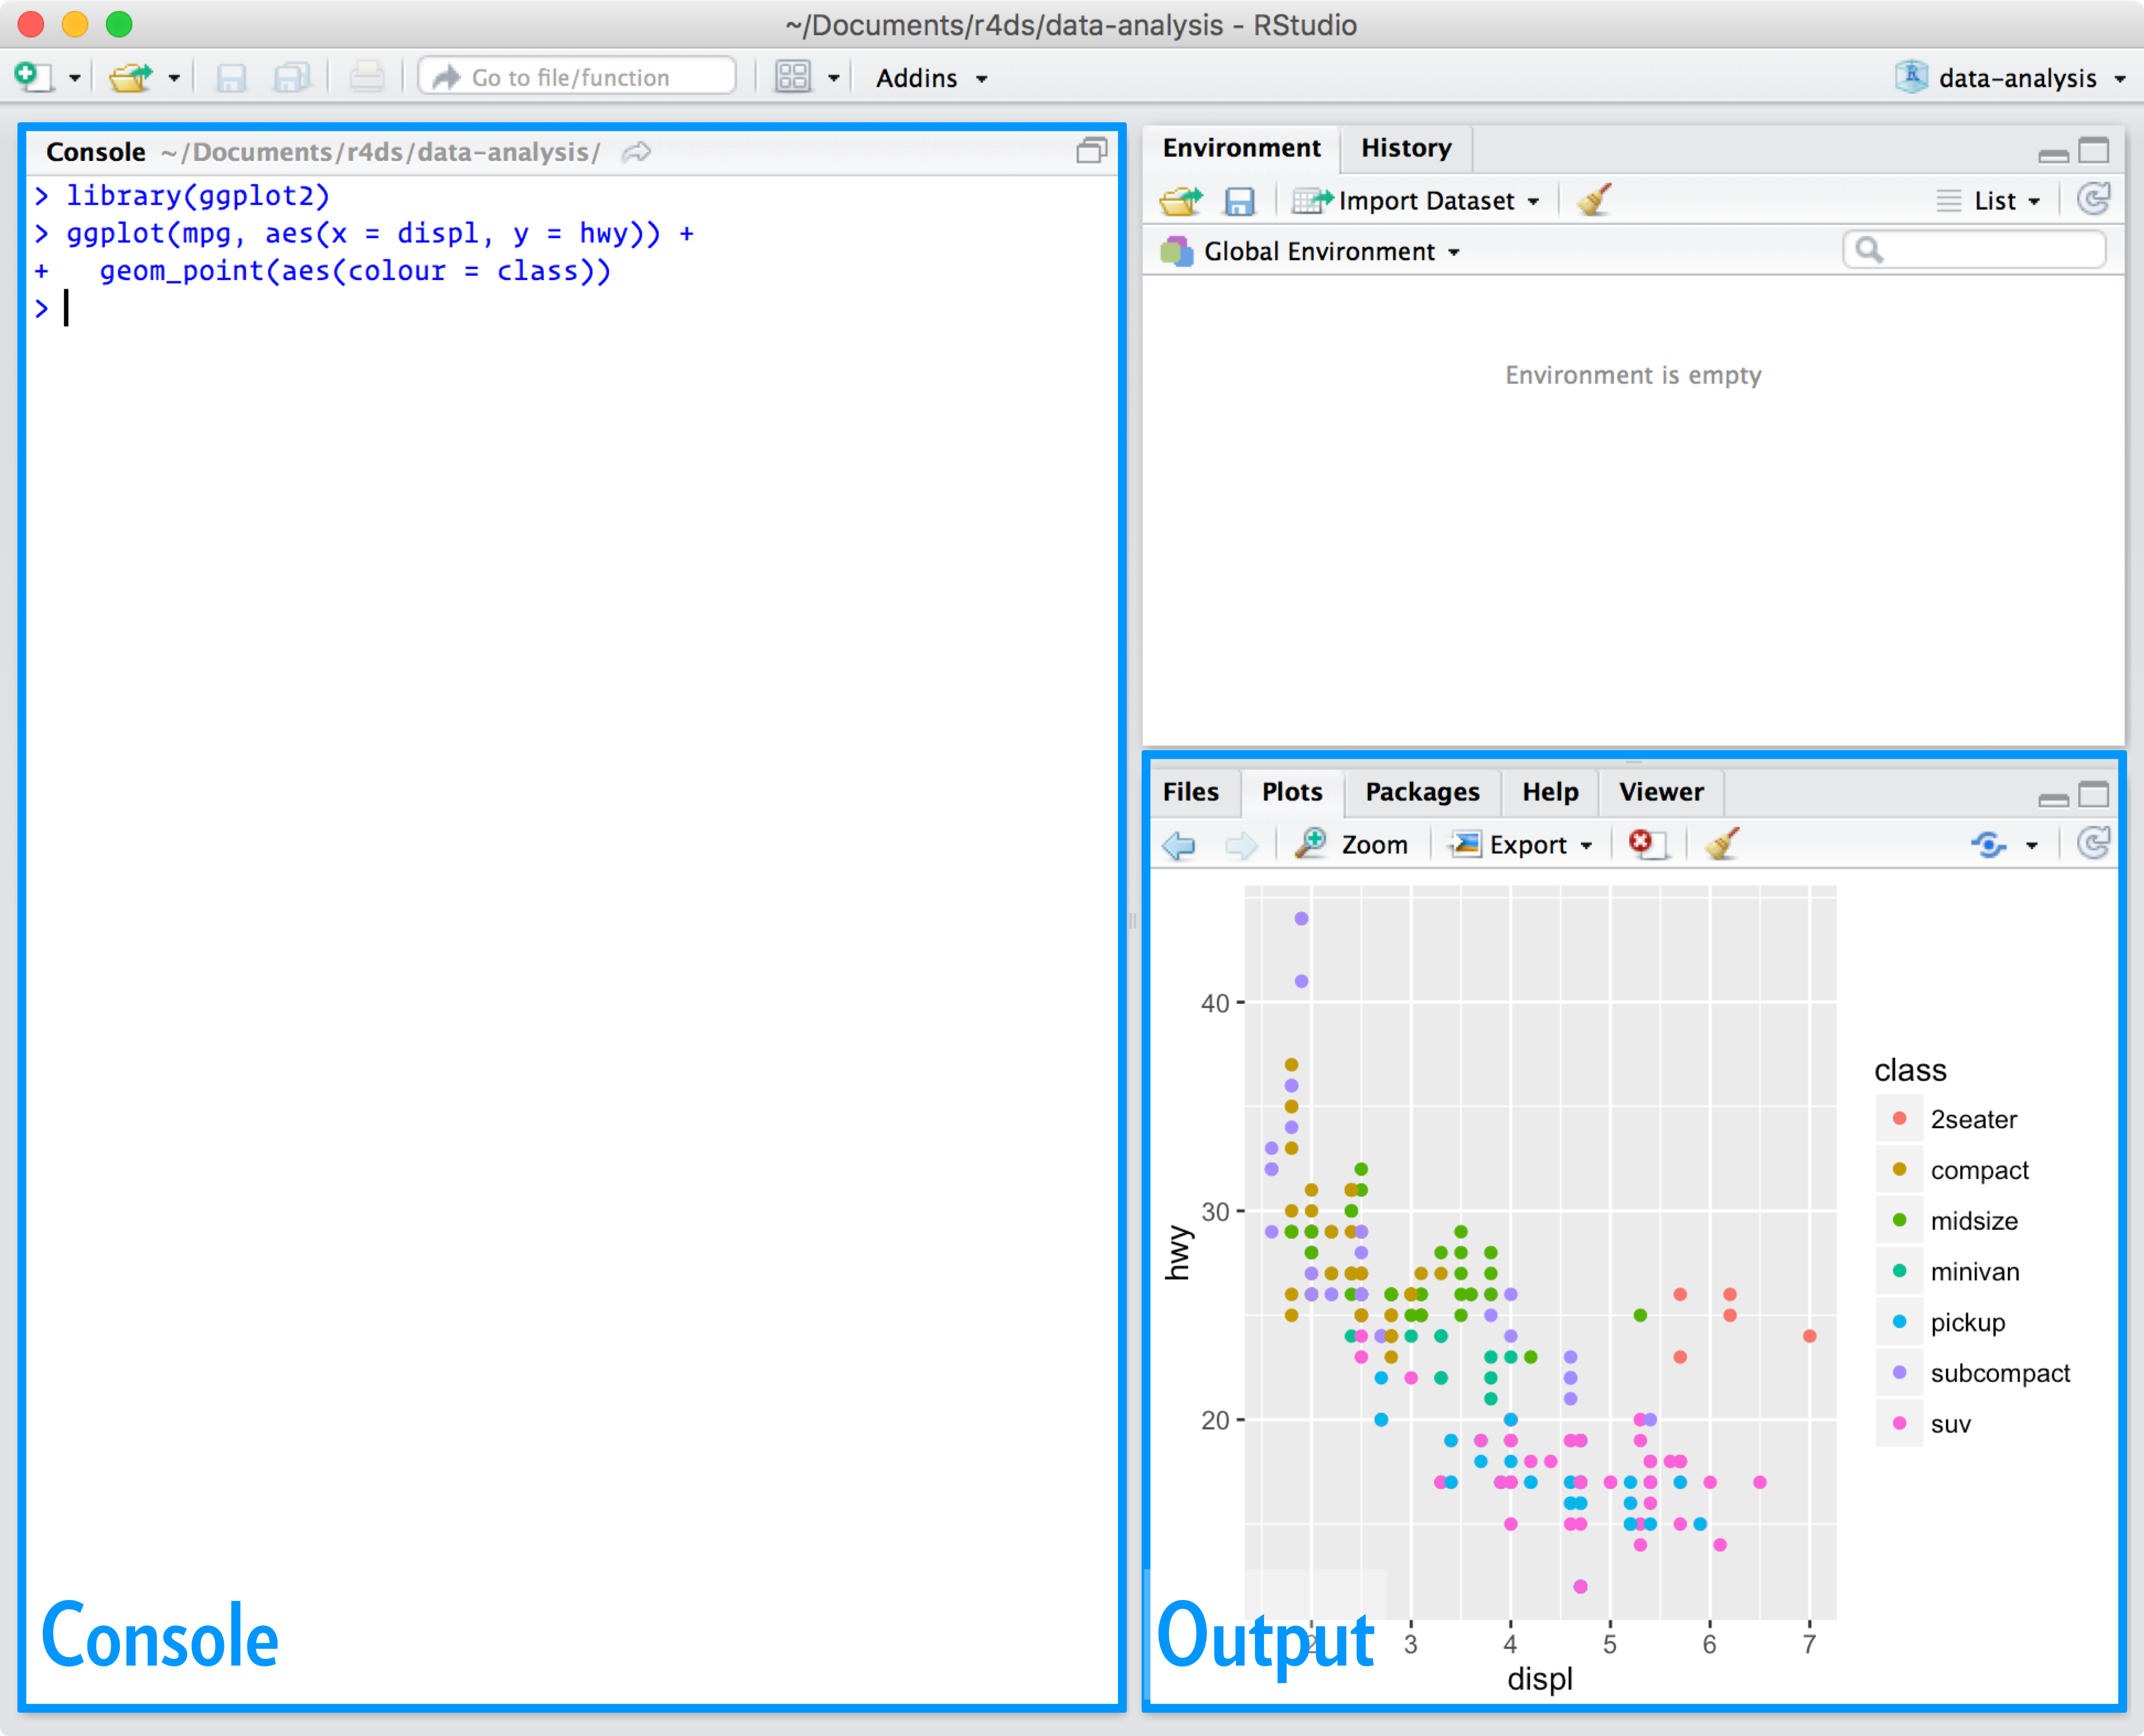
\includegraphics{rstudio-console.png}
\caption{}
\end{figure}

You can type R code into the \emph{Console} part of the user interface
and press the enter key to run them.

\subsection{R packages}\label{r-packages}

An R package is a collection of R code and documentation that can be
installed to enhance the standard R environment with additional
functionality. Currently, there are over ten thousand R packages
available on CRAN. Each of these R packages (mostly) aim to serve a
specific need, such as
\href{https://cran.r-project.org/web/packages/readxl/index.html}{reading
Excel spreadsheets},
\href{https://cran.r-project.org/web/packages/MODIStsp/index.html}{downloading
satellite imagery data},
\href{https://cran.r-project.org/web/packages/wdpar/index.html}{downloading
and cleaning protected area data}, or
\href{https://cran.r-project.org/web/packages/ENMeval/index.html}{fitting
environmental niche models}. In fact, R has such a diverse ecosystem of
R packages, that the question is (generally) not ``can I use R to do
\ldots{}?'' but ``what R package can I use to \ldots{}?''. During this
workshop, we will use various R packages. To install these R packages,
please run enter the code below in the \emph{Console} part of the
RStudio interface and press enter. Please note that you will require an
internet connection to install the packages and the installation process
may take a while to complete.

\begin{Shaded}
\begin{Highlighting}[]
\KeywordTok{install.packages}\NormalTok{(}\KeywordTok{c}\NormalTok{(}\StringTok{"sf"}\NormalTok{, }\StringTok{"tidyverse"}\NormalTok{, }\StringTok{"sp"}\NormalTok{, }\StringTok{"rgeos"}\NormalTok{, }\StringTok{"rgdal"}\NormalTok{, }\StringTok{"raster"}\NormalTok{,}
                   \StringTok{"prioritizr"}\NormalTok{, }\StringTok{"prioritizrdata"} \StringTok{"Rsymphony"}\NormalTok{, }\StringTok{"mapview"}\NormalTok{))}
\end{Highlighting}
\end{Shaded}

\section{Getting help}\label{getting-help}

There is a wealth of resources available for learning how to use R.
Although not required for this workshop, I would highly recommend that
you read \href{https://r4ds.had.co.nz/}{\emph{R for Data Science} by
Garrett Grolemund and Hadley Wickham}. \textbf{This veritable trove of R
goodness is freely available online.} If you spend a week going through
this book then you will save months debugging and rerunning incorrect
code. I would urge any and all ecologists -- especially those working on
Masters or PhD degrees -- to read this book. I even bought this book as
a Christmas present for my sister---and, yes, she was happy to receive
it! For intermediate users looking to skill-up, I would recommend the
\href{http://shop.oreilly.com/product/9781593273842.do}{\emph{The Art of
R Programming: A Tour of Statistical Software Design} by Norman Matloff}
and \href{https://adv-r.hadley.nz/}{\emph{Advanced R} by Hadley
Wickham}. Finally, if you wish to learn more about using R as a
geospatial information system (GIS), I would recommend
\href{https://geocompr.robinlovelace.net/}{\emph{Geocomputation with R}
by Robin Lovelace, Jakub Nowosad, and Jannes Muenchow} which is also
freely available online. I also recommend
\href{https://www.springer.com/gp/book/9781461476177}{\emph{Applied
Spatial Data Analysis} by Roger S. Bivand, Edzer Pebesmam and Virgilio
Gómez-Rubio} too.

\chapter{Introduction}\label{introduction}

The aim of this workshop is to help you get started with using the
prioritizr R package for systematic conservation planning. It is not
designed to give you a comprehensive overview and you will not become an
expert after completing this workshop. Instead, we want to help you
understand the core principles of conservation planning and guide you
through some of the common tasks involved with generating
prioritizations. Phrased provocatively, we want to give you the
knowledge base and confidence needed to start applying systematic
conservation planning to your own work.

One of the best ways, perhaps, to learn something new is to just give it
a go. As such, this workshop involves generating prioritizations for
protected area establishment and performing analyses to understand them.
This manual is divided into two main sections, the \textbf{Help} section
provides explanations and example R code for performing common
prioritization tasks (e.g.~importing data, creating target data, solving
conservation problems, calculating shortfalls) and the \textbf{Exercise}
section contains a systematic conservation planning case-study. During
this workshop, your aim is to work through the case-study in the
\textbf{Exercise} section and complete the tasks and answer the
questions. Since the \textbf{Exercise} section does not contain any R
code, you will need to read the \textbf{Help} section for information on
performing the tasks. This means that all of the code needed to complete
the \textbf{Exercise} section are in the \textbf{Help} section---you
just need to find them!

Finally, you are not alone in this workshop. If you are having trouble,
please put your hand up and one of the instructors will help you as soon
as they can. You can also ask the people sitting next to you for help
too. Please note that the first thing an instructor will ask you will
(probably) be ``what have you tried so far?''. This means that we can't
help you if you haven't tried anything.

\chapter{Data import and export}\label{data-import-and-export}

\begin{itemize}
\item
  How can I verify that I have entered the correct file path?

  \begin{itemize}
  \tightlist
  \item
    You can check that a file exists on your computer using the
    \texttt{file.exists} function. For instance, to check that the file
    \texttt{data.txt} exists, you can use
    \texttt{file.exists("data.txt")}.
  \end{itemize}
\item
  I am having trouble importing data, even though I am specifying the
  folder?

  \begin{itemize}
  \tightlist
  \item
    When we specify file paths on Windows systems, we use the
    \texttt{\textbackslash{}} character to delimit different folders.
    For instance, the complete file path for a file might be
    \texttt{C:\textbackslash{}Users\textbackslash{}kelly\textbackslash{}Downloads\textbackslash{}cost-data.tif}.
    However, R treats the \texttt{\textbackslash{}} character as a
    special character. This means that if you want to use the
    \texttt{\textbackslash{}} character, you need to specify it as
    \texttt{\textbackslash{}\textbackslash{}}. Thus if you want to refer
    to the file
    \texttt{C:\textbackslash{}Users\textbackslash{}kelly\textbackslash{}Downloads\textbackslash{}cost-data.tif}
    in an R environment, you need to specify it as
    \texttt{C:\textbackslash{}\textbackslash{}Users\textbackslash{}\textbackslash{}kelly\textbackslash{}\textbackslash{}Downloads\textbackslash{}\textbackslash{}cost-data.tif}.
  \end{itemize}
\item
  How can I import spatial raster data?

  \begin{itemize}
  \tightlist
  \item
    Spatial raster data (e.g. .asc and .tif files) can be imported using
    the \texttt{stack} function from the raster R packages. For example,
    if the file name for your raster data was called
    \texttt{cost-data.tif} then you could import it using
    \texttt{"cost\_data\ \textless{}-\ stack("cost-data.tif")}. Note
    that you will probably need to specify the folder path for the file
    too. For example, if you downloaded the file to the Downloads folder
    on your computer, then you might need to use something like this
    \texttt{"cost\_data\ \textless{}-\ stack("C:\textbackslash{}\textbackslash{}Users\textbackslash{}\textbackslash{}kelly\textbackslash{}\textbackslash{}Downloads\textbackslash{}\textbackslash{}cost-data.tif")"}
    depending on your system user name.
  \end{itemize}
\item
  How can I import spatial vector data?

  \begin{itemize}
  \tightlist
  \item
    Spatial vector data (e.g.~shapefiles) can be imported using the
    \texttt{readOGR} function in the rgdal R package. For example, if
    the file name for your shapefile was \texttt{animals.shp}, then you
    could import it using
    \texttt{animal\_data\ \textless{}-\ readOGR("animals.shp")}. Note
    that you will probably need to specify the folder path for the file
    too. For example, if you downloaded the file to the Downloads folder
    on your computer, then you might need to use something like this
    \texttt{"cost\_data\ \textless{}-\ stack("C:\textbackslash{}\textbackslash{}Users\textbackslash{}\textbackslash{}frank\textbackslash{}\textbackslash{}Downloads\textbackslash{}\textbackslash{}animals.tif")"}
    depending on your system user name.
  \end{itemize}
\item
  How can I import spreadsheet data?
\item
  How can I export spatial raster data?
\item
  How can I export spatial vector data?
\item
  How can I export spreadsheet data?
\end{itemize}

\chapter{Gap analysis}\label{gap-analysis}

TODO

\chapter{Minimum set problem}\label{min-set}

TODO

\chapter{Minimum shortfalls problem}\label{min-shortfalls}

TODO

\chapter{Maximum features problem}\label{max-features}

TODO

\chapter{Maximum phylogenetic diversity problem}\label{max-phylo-div}

TODO

\chapter{Tasks}\label{tasks}

TODO

\chapter{Error glossary}\label{error-glossary}

If you are having trouble running a specific line of code or a function,
then one of the best ways to find help is to read (i) the error message
and (ii) the documentation. Believe it or not, a human actually wrote
the function that is throwing that (probably) annoying and (probably)
indecipherable error message and they (almost always) genuinely want to
help you. Instead of (or in addition to) getting frustrated at an error,
you might choose to appreciate the fact that someone went to the trouble
of writing additional code so that a description of what went wrong
would be displayed. Indeed, since there are an unlimited numbers of ways
that code can be incorrect, throwing a short and precise error message
is actually helpful because it tells you \emph{what went wrong} rather
than \emph{potentially incorrectly guessing what should be fixed}. After
reading the error message, take the time to think about what it means.
Debugging is the process of iterating through each and every assumption
that you made until you identify which of your assumptions is incorrect.
This is liberating because it means it is within your power to fix the
code. When reading an error message, try to interpret each word
individually -- you might have to google technical terms to understand
them, that's OK -- and then put them together to try to understand what
they mean together. For instance, consider the code below:

\begin{Shaded}
\begin{Highlighting}[]
\KeywordTok{read.table}\NormalTok{(}\StringTok{"fred.txt"}\NormalTok{)}
\end{Highlighting}
\end{Shaded}

\begin{verbatim}
## Warning in file(file, "rt"): cannot open file 'fred.txt': No such file or
## directory
\end{verbatim}

\begin{verbatim}
## Error in file(file, "rt"): cannot open the connection
\end{verbatim}

This tells us that R \texttt{cannot\ open\ the\ connection} to the file
\texttt{"fred.txt"} because \texttt{No\ such\ file\ or\ directory} was
found. Now we have to think of all the reasons why this could be true.
Is it possible that we have misspelled the filename? Perhaps we meant
\texttt{"fed.txt"}, \texttt{"fran.txt"}, or \texttt{"fred.csv"}? Or
perhaps we need to specify a folder name, such as
\texttt{"data/fred.txt"}? Or maybe we forgot to save the data after
entering it into Excel?

Now let us consider another example:

\begin{Shaded}
\begin{Highlighting}[]
\NormalTok{a <-}\StringTok{ }\DecValTok{1}
\NormalTok{b <-}\StringTok{ "c"}
\NormalTok{a }\OperatorTok{+}\StringTok{ }\NormalTok{b}
\end{Highlighting}
\end{Shaded}

\begin{verbatim}
## Error in a + b: non-numeric argument to binary operator
\end{verbatim}

This error message is a bit more cryptic---but it mentions something
about a \texttt{non-numeric\ argument}. This would indicate that
something went wrong because something was not a number. If we look at
the code, can we see something that is not a number? Yes, \texttt{c} is
not a number. It is a character-type object (i.e. \texttt{"k"}). Does it
make sense to add the letter ``k'' to the number 1? Well, not in R. If
we wanted to create the character \texttt{"c1"} we would have to use a
function designed for this purpose (e.g. \texttt{paste}). Alternatively,
if we wanted to employ the hexadecimal numeral system, where letters
count as numbers, then we would need to specify this.

Let's look at another example:

\begin{Shaded}
\begin{Highlighting}[]
\NormalTok{d <-}\StringTok{ }\KeywordTok{c}\NormalTok{(}\StringTok{"a"}\NormalTok{, }\StringTok{"b, "}\NormalTok{c}\StringTok{")}
\end{Highlighting}
\end{Shaded}

\begin{verbatim}
## Error: <text>:1:18: unexpected symbol
## 1: d <- c("a", "b, "c
##                      ^
\end{verbatim}

This error message mentions an \texttt{unexpected\ symbol}. If a symbol
is unexpected, then this would suggest that the our error is occurring
because we have typed an additional symbol or are missing a symbol. If
we carefully look at the code for missing symbols, we can see that we
are missing a quote (\texttt{"}) symbol after after the \texttt{b}.

\bibliography{references.bib}


\end{document}
